\documentclass{beamer}
\mode<presentation>
\usepackage[utf8]{inputenc}

\usetheme{Dresden}
\usecolortheme{beaver}
\setbeamertemplate{footline}[frame number]
\setbeamertemplate{caption}[numbered]
\setbeamertemplate{navigation symbols}{}
\usepackage[english]{babel}%Set language as english%
\usepackage[babel]{csquotes}%Nicer quotations%
\usepackage{indentfirst}
\usepackage[protrusion=true,expansion=true]{microtype}
\usepackage{enumitem}%Different enumeration options%
%Math Formatting%
\usepackage{amsmath}%AMS Math%
\usepackage{amsthm}%Theorem Formatting%
\usepackage{amssymb}%AMS Symbols%
\usepackage{array}%Allows for more complex matrices
\usepackage{siunitx}%Formats SI units%
\DeclareSIUnit{\molar}{M}%Adds molarity as unit%
\usepackage{booktabs}%Typsets tables%
\newcommand{\specialcell}[2][c]{\begin{tabular}[#1]{@{}l@{}}#2\end{tabular}}
\newcommand{\specialcellbold}[2][c]{%
	\bfseries
	\begin{tabular}[#1]{@{}l@{}}#2\end{tabular}%
}
\usepackage{chemformula}%Typsets Chemical Formulas$
%Image Formatting%
\usepackage{graphicx}%Enchanced graphics support%
\usepackage{media9}
\graphicspath{{../figures/}}
\usepackage{float}%Float options$

\usepackage[
backend=biber,
style=chem-acs
]{biblatex}
\addbibresource{references.bib}

\usetheme{default}

\title{Parallels Between Chemical Oscillation and Discrete Time Economic Growth Models}
\author{Benjamin Bui}
\date{October 5, 2018}
\begin{document}
\begin{frame}
	\titlepage
\end{frame}

\begin{frame}
	\frametitle{Overview}
	\tableofcontents
\end{frame}

\section{Introduction}
\begin{frame}{Motivation}
	Can we apply techniques used in studying chemical oscillations and physical dynamical systems to analyze economic models?
\end{frame}

\begin{frame}{Key Differences}
	\begin{itemize}
		\item
			Physical laws make up the foundations of chemical systems

		\item
			Macroscale physical systems operate in continuous time
	\end{itemize}
\end{frame}

\begin{frame}{Natural Discrete Time Systems}
	\begin{columns}
		\begin{column}{0.5\textwidth}
			\begin{itemize}
					\item
						Ecological systems are often modelled using discrete time equations

					\item
						One classically used system is the logistic map\autocite{Maier2010}
					\item
						The continuous time analogue is used to model autocatalytic reactions
				\end{itemize}
		\end{column}
		\begin{column}{0.5\textwidth}
			\begin{figure}
				\centering
				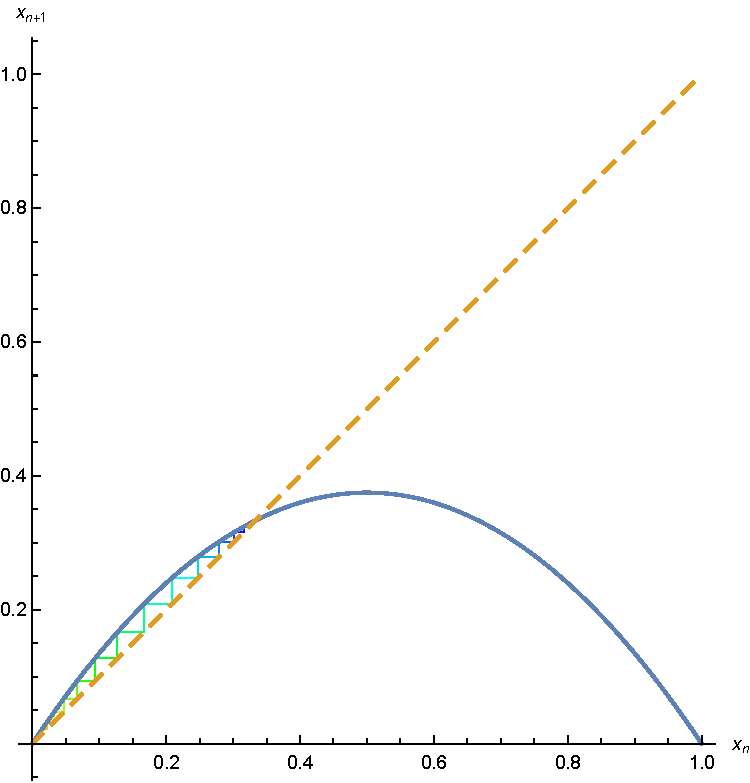
\includegraphics[width=\textwidth]{logistic.eps}
			\end{figure}
		\end{column}
	\end{columns}
\end{frame}

\section{The Framework}
\begin{frame}{Background}
	\begin{columns}
		\begin{column}{0.5\textwidth}
			\begin{itemize}
					\item
						John Maynard Keynes

					\item
						Paul Samuelson and Hicks attempted to formalize a business cycle model\autocite{Puu2003}
				\end{itemize}
		\end{column}
		\begin{column}{0.5\textwidth}
			\begin{figure}
				\centering
				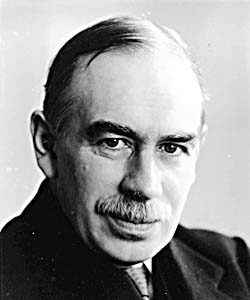
\includegraphics[width=\textwidth]{keynes.jpg}
			\end{figure}
		\end{column}
	\end{columns}
\end{frame}

\begin{frame}{Investment}
	\begin{columns}
		\begin{column}{0.5\textwidth}
				\begin{itemize}
					\item
						Capital stock is in a given proportion of production\autocite{Press1939}

					\item
						Hicks and Goodwin changed the linear relationship to a hyperbolic tangent curve
					\item
						This curve can be approximated with a linear-cubic Taylor series expansion
				\end{itemize}
		\end{column}
		\begin{column}{0.5\textwidth}
			\begin{figure}
				\centering
				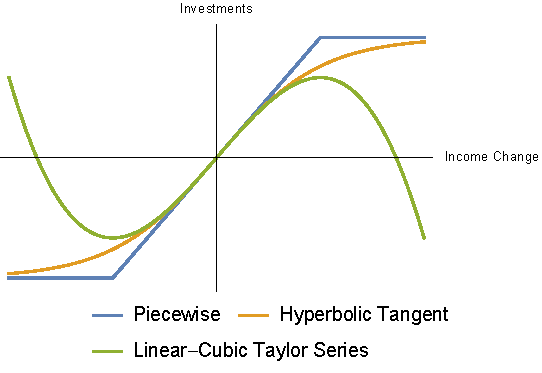
\includegraphics[width=\textwidth]{investment_curve.eps}
			\end{figure}
		\end{column}
	\end{columns}
\end{frame}

\begin{frame}{Investment}
	\begin{equation*}
		I_t=v(Y_{t-1}-Y_{t-2})-v(Y_{t-1}-Y_{t-2})^3
	\end{equation*}
\end{frame}

\begin{frame}{Consumption}
	\begin{columns}
		\begin{column}{0.5\textwidth}
			\begin{itemize}
				\item
					Suppose consumption is a two-period process
				\item
					All production goes towards consumption and investments
			\end{itemize}
		\end{column}

		\begin{column}{0.5\textwidth}
			\begin{gather*}
				C_t=(1-s)Y_{t-1}+sY_{t-2}\\
				Y_t=C_t+I_t
			\end{gather*}
		\end{column}
	\end{columns}
\end{frame}

\begin{frame}{Production}
	\begin{columns}
		\begin{column}{0.3\textwidth}
			\centering
			Insert the functions for investment and consumption into production
		\end{column}
		\begin{column}{0.7\textwidth}
			\begin{itemize}
				\item
					\begin{equation*}
						\begin{split}
						Y_t-Y_{t-1}=(v-s)(Y_{t-1}-Y_{t-2})\\
						-v(Y_{t-1}-Y_{t-2})^3
					\end{split}
					\end{equation*}

				\item
					\begin{equation*}
						Z_{t-1}\equiv Y_{t}-Y_{t-1}
					\end{equation*}

				\item
					\begin{equation*}
						Z_t=(v-s)Z_{t-1}-vZ^3_{t-1}
					\end{equation*}
			\end{itemize}
		\end{column}
	\end{columns}
\end{frame}

\begin{frame}{A Little Economic Trickery}
	\begin{columns}
		\begin{column}{0.5\textwidth}
			\begin{itemize}
				\item
					\(v\) can be any arbitrary value by rescaling how we measure income
				\item
					This allows the function to be contained in a box of interval \([-1,1]\)
			\end{itemize}
		\end{column}
		\begin{column}{0.5\textwidth}
			\begin{itemize}
				\item
					\begin{equation*}
						\mu\equiv(v-s)
					\end{equation*}

				\item
					\begin{equation*}
						Z_t=\mu Z_{t-1}-(\mu+1)Z^3_{t-1}
					\end{equation*}
			\end{itemize}
		\end{column}
	\end{columns}
\end{frame}

\section{Quantitative Analysis}
\begin{frame}{Fixed Point Stability}
	\begin{itemize}
		\item
			\textbf{Fixed Points}\hspace{5cm} \textbf{Stability}
		\item
			\begin{equation*}
				Z=0 \hspace{5cm} \lvert \mu \rvert<1
			\end{equation*}

		\item
			\begin{equation*}
				Z=\pm\sqrt{\frac{\mu-1}{\mu+1}} \hspace{4cm} 1<\mu<2
			\end{equation*}
	\end{itemize}
\end{frame}

\begin{frame}{Fixed Point Stability}
	\begin{figure}
		\centering
		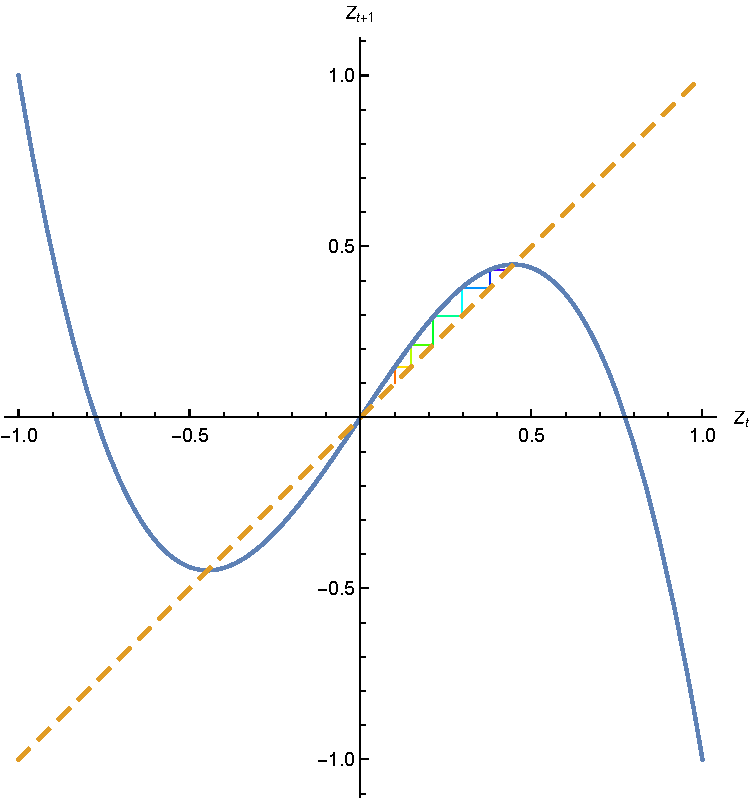
\includegraphics[height=0.9\textheight]{fixed_point.eps}
	\end{figure}
\end{frame}

\begin{frame}{Cyclic Behavior}
	\begin{columns}
		\begin{column}{0.5\textwidth}
			\begin{figure}
				\centering
				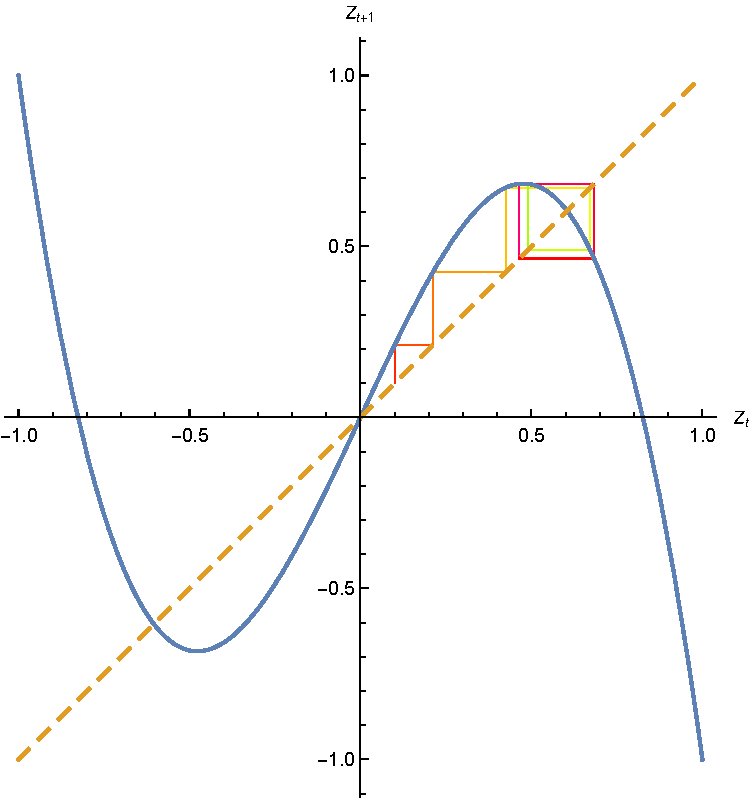
\includegraphics[height=0.8\textwidth,width=0.8\textwidth]{2_cycle.eps}
			\end{figure}
		\end{column}
		\begin{column}{0.5\textwidth}
			\begin{figure}
				\centering
				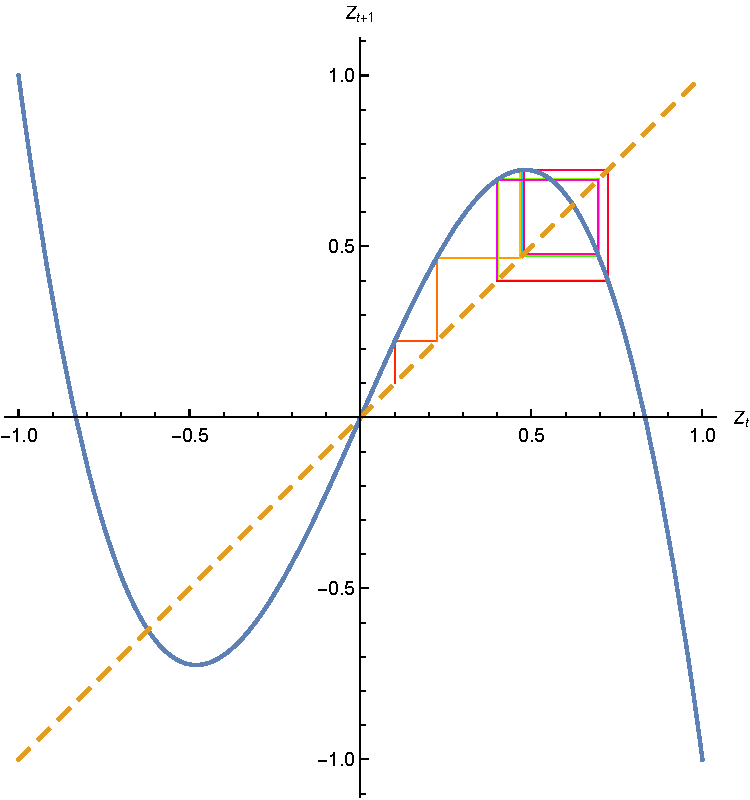
\includegraphics[height=\textwidth,width=0.8\textwidth]{8_cycle.eps}
			\end{figure}
		\end{column}
	\end{columns}
\end{frame}

\begin{frame}{Confined Chaos}
	\begin{columns}
		\begin{column}{0.5\textwidth}
			\begin{itemize}
				\item
					\centering
					Occurs when parameter reaches Feigenbaum point

				\item
					\begin{equation*}
						\mu\approx2.302
					\end{equation*}
			\end{itemize}
		\end{column}
		\begin{column}{0.5\textwidth}
			\begin{figure}
				\centering
				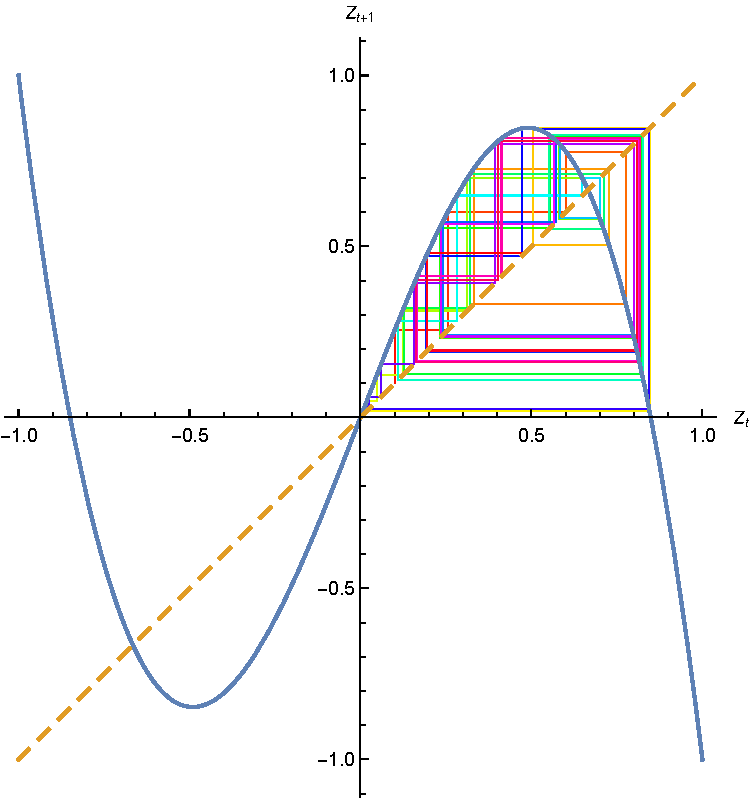
\includegraphics[width=\textwidth]{contained_chaos.eps}
			\end{figure}
		\end{column}
	\end{columns}
\end{frame}

\begin{frame}{Spillover Chaos}
	\begin{columns}
		\begin{column}{0.5\textwidth}
			\begin{itemize}
				\item
					\centering
					Occurs once extremum of the cubic marginally exceed where the cubic has a zero

				\item
					\begin{gather*}
						f^\prime(Z)=\mu-3(\mu+1)Z^2=0\\
						Z=\pm\sqrt{\frac{\mu}{\mu+1}}\\
						\mu>\frac{3\sqrt{3}}{2}\approx2.5981
					\end{gather*}
			\end{itemize}
		\end{column}

		\begin{column}{0.5\textwidth}
			\begin{figure}
				\centering
				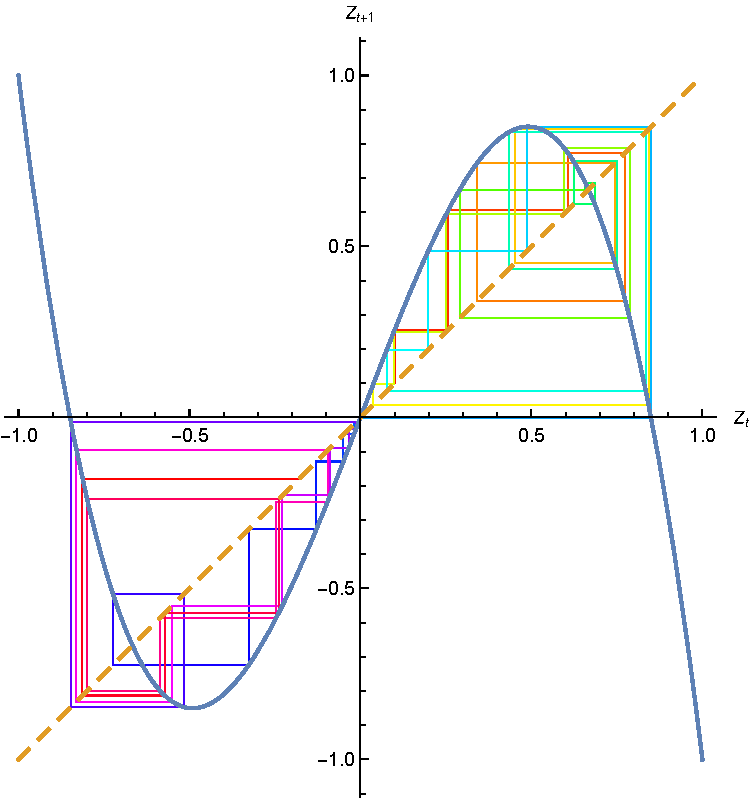
\includegraphics[width=\textwidth]{spillover_chaos.eps}
			\end{figure}
		\end{column}
	\end{columns}
\end{frame}

\begin{frame}{True Cyclic Economy}
	\begin{columns}
		\begin{column}{0.5\textwidth}
				There are windows of order in chaotic regions
		\end{column}
		\begin{column}{0.5\textwidth}
			\begin{figure}
				\centering
				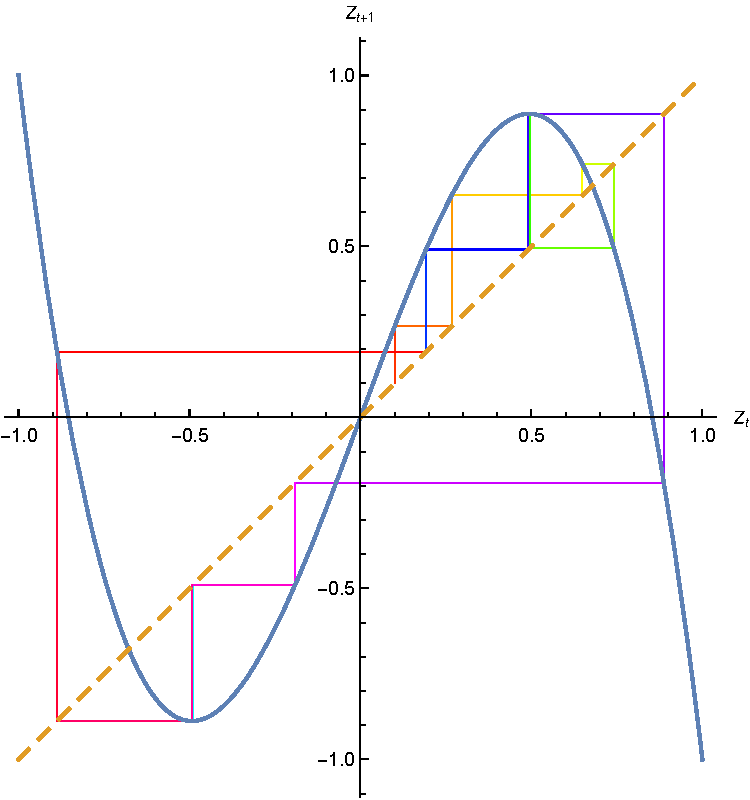
\includegraphics[width=\textwidth]{spillover_cycle.eps}
			\end{figure}
		\end{column}
	\end{columns}
\end{frame}

\begin{frame}{Exploding Solutions}
	\begin{columns}
		\begin{column}{0.5\textwidth}
			\begin{itemize}
				\item
					Occur once the cubic escapes the box
				\item
					\begin{equation*}
						\mu>3
					\end{equation*}
			\end{itemize}
		\end{column}
		\begin{column}{0.5\textwidth}
			\begin{figure}
				\centering
				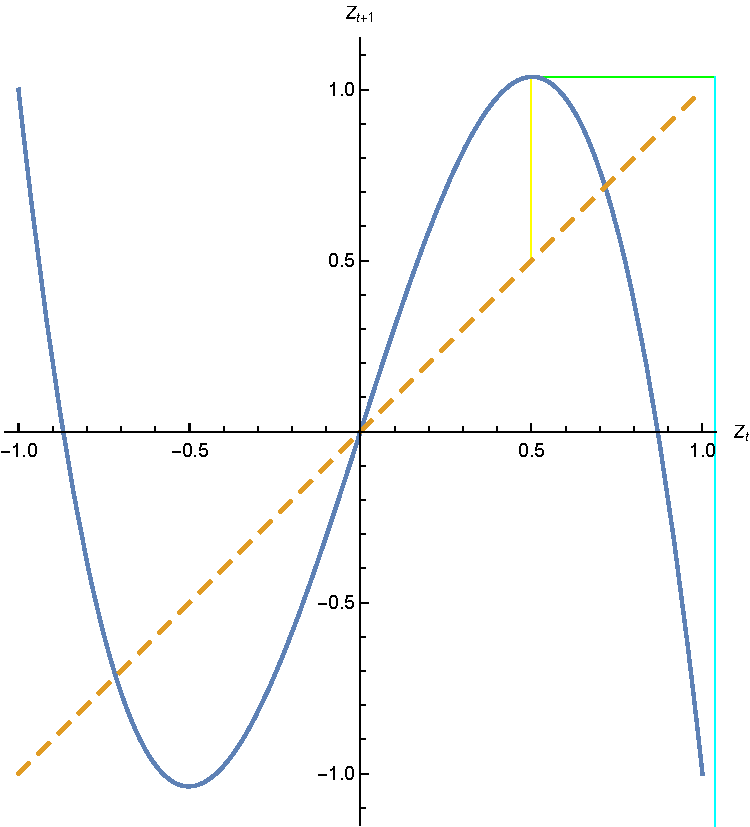
\includegraphics[width=\textwidth]{exploding.eps}
			\end{figure}
		\end{column}
	\end{columns}
\end{frame}

\begin{frame}{Bifurcations and the Lyapunov Exponent}
	\begin{columns}
		\begin{column}{0.5\textwidth}
			\begin{itemize}
				\item
					A way to visualize progression of stability
				\item
					\begin{equation*}
						L(Z_0)=\lim\limits_{n\to\infty}\frac{1}{n}\sum\limits_{i=1}^{i=n}\ln\lvert f^\prime(Z_{i-1}\rvert)
					\end{equation*}
			\end{itemize}
		\end{column}
		\begin{column}{0.5\textwidth}
			\begin{figure}
				\centering
				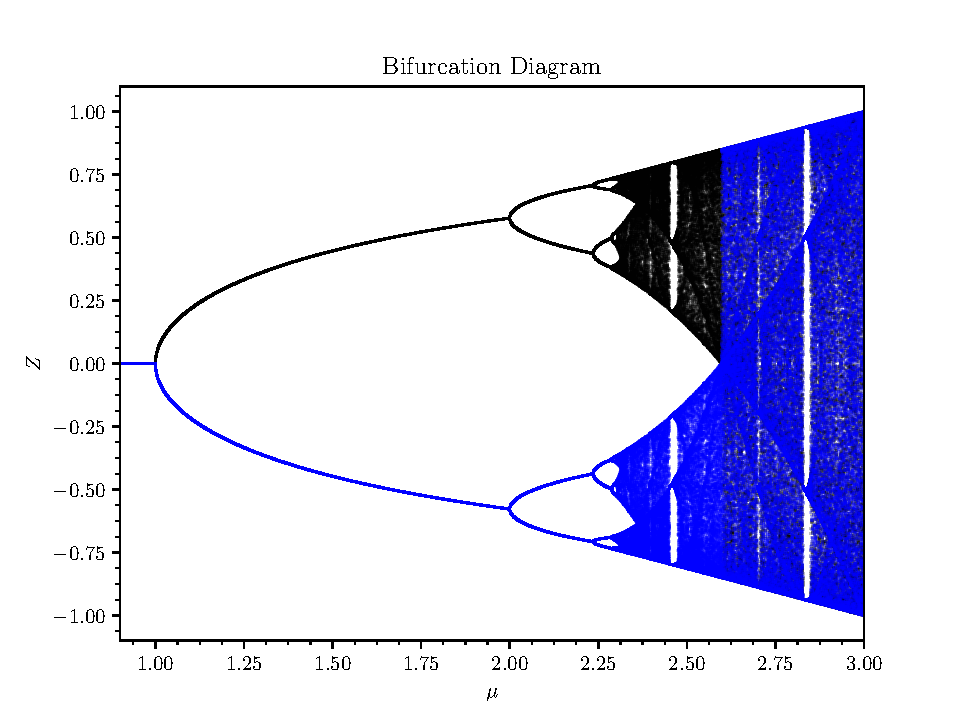
\includegraphics[height=0.4\textheight]{bifurcation.eps}
			\end{figure}
			\begin{figure}
				\centering
				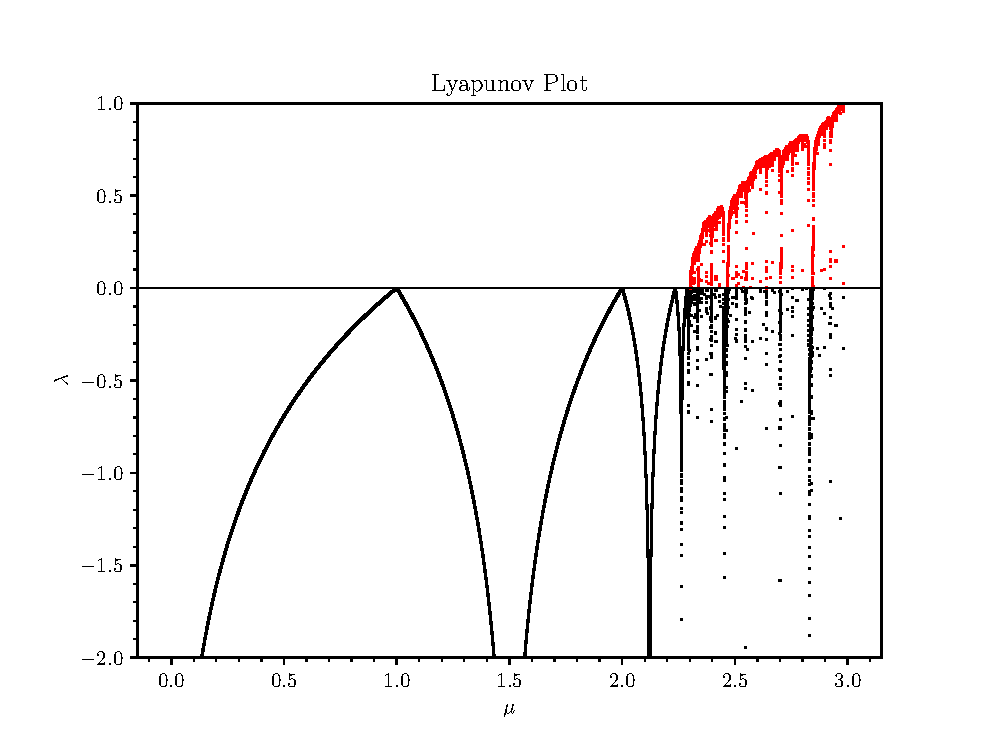
\includegraphics[height=0.3\textheight]{lyapunov.eps}
			\end{figure}
		\end{column}
	\end{columns}
\end{frame}

\section*{Next Steps}
\begin{frame}{Next Steps}
	\begin{columns}
		\begin{column}{0.5\textwidth}
			\begin{itemize}
				\item
					Samuelson-Hicks is a very simplified model

				\item
					There are a variety of variables and mechanism that are unnacounted for

				\item
					Kaldor and Solow-Swann
			\end{itemize}
		\end{column}
		\begin{column}{0.5\textwidth}
			\begin{figure}
				\centering
				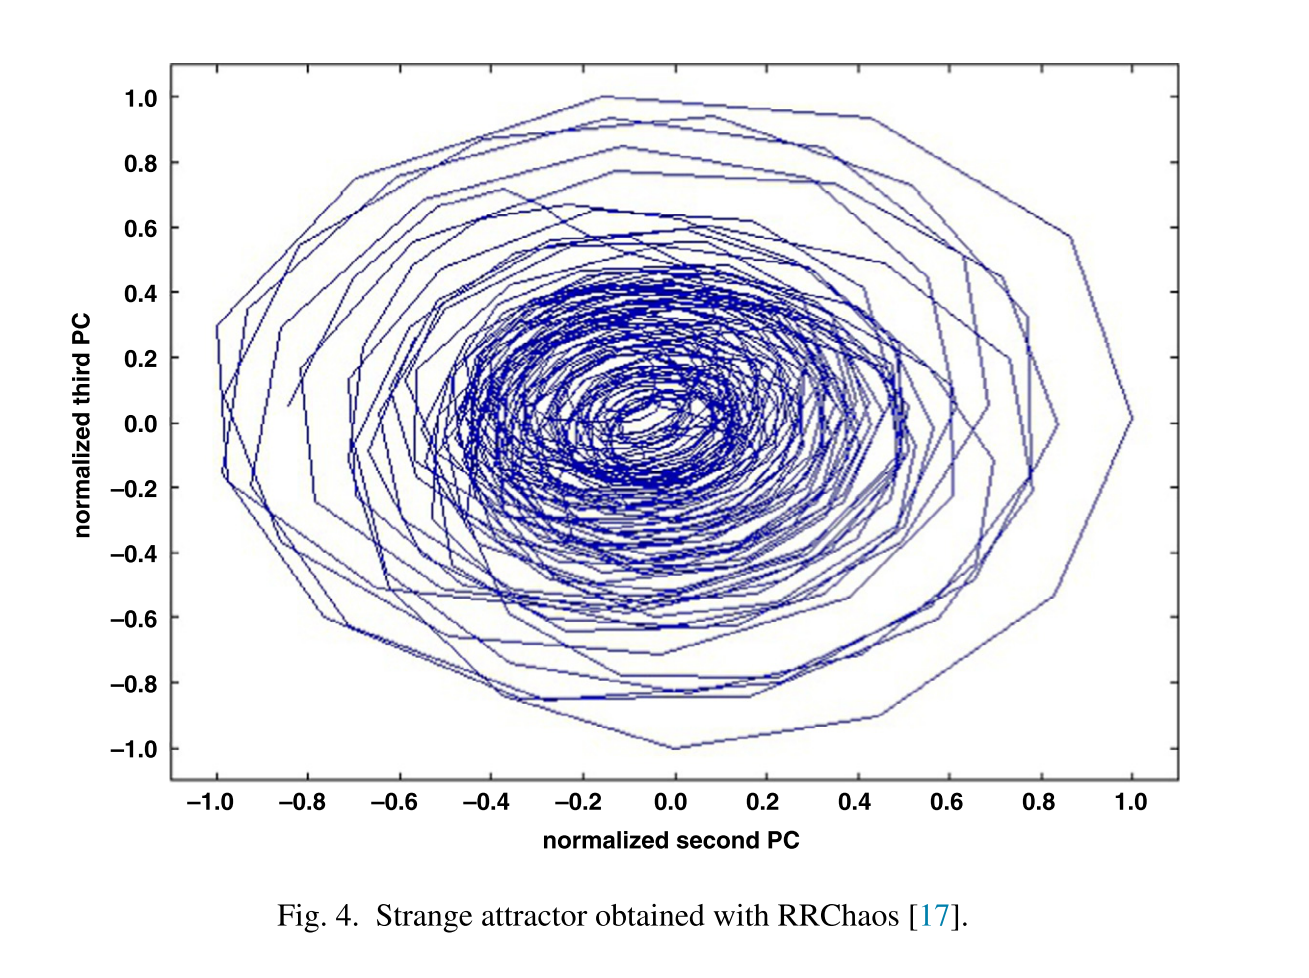
\includegraphics[width=\textwidth]{kaldor.png}
			\end{figure}
		\end{column}
	\end{columns}
\end{frame}

\begin{frame}[allowframebreaks]{References}
	\nocite{*}
	\printbibliography
\end{frame}
\end{document}
